\documentclass{report}
\usepackage[italian]{babel}
\usepackage[utf8]{inputenc}
\usepackage{natbib}
\usepackage{graphicx}
\usepackage{cleveref}

\title{
    Titolo Progetto \\
    \large Applicazioni e Servizi Web
}

\author{Federico Pettinari - 988120 \{federico.pettinari2@studio.unibo.it\}\\
Hamado Dene - 973128 \{hamado.dene@studio.unibo.it\}}
\date{\today}

\begin{document}

\maketitle
\section{Introduzione}
Introduzione \citep{adams1995hitchhiker}

\section{Requisiti}
\begin{itemize}
    \item Progettare e sviluppare una web app per la visualizzazione e gestione dei dati sui rifiuti cittadini
    \item I cassonetti sono dotati di sensore di peso e lettore rfid per identificare l’utente che sta conferendo i rifiuti
    \item La piattaforma delle calcolare il costo mensile in funzione del tipo di rifiuto e peso.
    \item Deve mostrare la notifica del conferimento all’utente
    \item Deve mostrare grafici statistici sul conferimento
\end{itemize}

\section{Design}
\subsection{Architettura}
L'architettura è raffigurata in \Cref{fig:arch}.
Ogni richiesta HTTP viene ricevuta e smistata dal reverse proxy.
Le chiamate che iniziano con /api vengono passate al backend, mentre le altre al frontend.
Questo aiuta a separare frontend e backend in modo trasparente e senza bisogno di utilizzare Cross-Origin Resource Sharing (CORS).

\begin{figure}[h!]
\centering
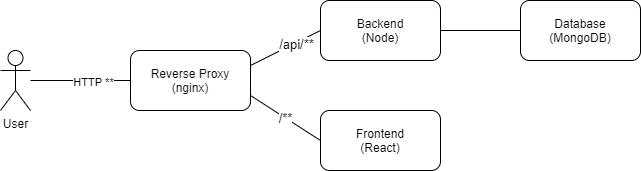
\includegraphics[width=\textwidth]{arch}
\caption{Architettura}
\label{fig:arch}
\end{figure}

\subsection{Interfaccia utente}
TODO. Mockup....

\section{Tecnologie}
Il progetto utilizza le seguenti tecnologie:
\begin{itemize}
    \item Docker - per disaccoppiare il software dal sistema operativo e facilitarne il porting ed installazione.
    \item MongoDB - database non relazionale di documenti
    \item Node - come server web sia per frontend e backend
    \item Express - libreria per gestire chiamate e route HTTP
    \item Mongoose - come libreria di object modeling per mongodb
    \item Mocha e Supertest - per testing automatizzato nel backend
    \item mongodb-memory-server - per utilizzare un database mongodb in memoria, in modo da velocizzare l'esecuzione dei test
    \item bcrypt - per criptare le password degli utenti ai fini di sicurezza
    \item express-jwt - libreria per facilitare l'uso di tokens JWT utilizzati nel sistema di login utente
    \item Nodemon - tool che riavvia le applicazioni Node ad ogni modifica del sorgente
    per velocizzarne lo sviluppo e debugging
    \item React - framework per frontend
    \item SCSS - libreria pre-processore di CSS per facilitarne il riuso
\end{itemize}

\section{Codice}
Solo aspetti rilevanti.

\section{Test}
Test effettuati sul codice e test con utenti.

\section{Deployment}
Rilascio, installazione e messa in funzione.


\section{Conclusioni}
Conclusioni

\bibliographystyle{plain}
\bibliography{references}
\end{document}
